\documentclass{beamer}

\mode<presentation>
{
  \usetheme{boxes}      
  \usecolortheme{whale} 
  \usefonttheme{serif} 
  \setbeamertemplate{navigation symbols}{}
  \setbeamertemplate{caption}[numbered]
} 
\usepackage{tikz}
\setbeamercovered{highly dynamic}
\newcounter{saveenumi}
\newcommand{\seti}{\setcounter{saveenumi}{\value{enumi}}}
\newcommand{\conti}{\setcounter{enumi}{\value{saveenumi}}}
\renewcommand{\thefigure}{\thesection-\arabic{figure}}
\usetikzlibrary{shapes.geometric,calc,angles,positioning,intersections,quotes,decorations,babel,patterns,fit}
\usepackage{tkz-euclide}
\usetkzobj{all}
\usepackage[english]{babel}
\usepackage[utf8]{inputenc}
\usepackage[T1]{fontenc}
\usepackage{graphics}
\usepackage{standalone}
\usepackage{gensymb}
\usepackage{amsmath}
\title[Your Short Title]{Exercises}
\author{Durga Prasad}
\institute{}
\date{22 December 2019}
\begin{document}
\begin{frame}
  \titlepage
\end{frame}
\begin{frame}{Triangle exercise}
\begin{enumerate}
\item ABC and AMP are two right triangles, right
angled at B and M respectively. M lies on AC
and AB is extended to meet P. Prove that:
\seti
\begin{enumerate}
\item $\triangle{ABC} \sim \triangle{AMP}$
\item $\frac{CA}{PA}=\frac{BC}{MP}$
\end{enumerate}
\end{enumerate}
\textbf{Solution:}

\begin{figure}[!ht]
\resizebox{.4\linewidth}{!}
{
\documentclass{article}
\usepackage{tikz}
\usetikzlibrary{shapes.geometric,calc,angles,positioning,intersections,quotes,decorations,babel,patterns,fit}
\usepackage{tkz-euclide}
\usetkzobj{all}
\begin{document}
\begin{tikzpicture}[scale =1.5,>=stealth,point/.style = {draw, circle, fill = black, inner sep = 1pt},]
\node (C) at (8,7.8)[point,label=above :$C$] {};
\node (A) at (0,0)[point,label=below :$A$] {};
\node (B) at (8,0)[point,label=below :$B$] {};
\node (P) at (10,0)[point,label=below :$P$] {};
\node (M) at (5,4.9)[point,label=above :$\textbf{M}$] {};
\draw (A)--(B);
\draw (B)--(C);
\draw (C)--(A);
\draw (P)--(M);
\draw (B)--(P);
\tkzMarkAngle[fill=black!40,size=0.5cm,mark=](C,B,A)
\tkzLabelAngle[pos=0.65](A,C,B){}
\tkzMarkAngle[fill=black!40,size=0.5cm,mark=](A,M,P)
\tkzLabelAngle[pos=0.65](A,C,B){}
\end{tikzpicture}
\end{document}
}
\caption{right angled triangles}
\label{fig:foo}
\end{figure}
\end{frame}
\begin{frame}
From the above figure
\begin{align}
	\angle{CAB} =\angle{MAP} \\
	\angle{ABC} = \angle{AMP}
\end{align}
From 1 and 2
\begin{align}
\triangle{ABC} \sim \triangle{AMP}
\end{align}
\begin{itemize}
\item As correspondinng sides are proportional
$\frac{CA}{PA}=\frac{BC}{MP}=\frac{AB}{AM}$

\begin{center}
$\frac{CA}{PA}=\frac{BC}{MP}$
\end{center}
\end{itemize}
\end{frame}
\begin{frame}{Triangle construction}
\begin{enumerate}
\conti
\item In $\triangle{ABC}$ ,a=8,$\angle{B}=45\degree$ and c-b=3.5. Sketch $\triangle{ABC}$
\seti
\end{enumerate}
\textbf{Solution:}
\begin{figure}[!ht]
\resizebox{0.3\linewidth}{!}
{
\documentclass{article}
\usepackage{tikz}
\usetikzlibrary{shapes.geometric,calc,angles,positioning,intersections,quotes,decorations,babel,patterns,fit}
\usepackage{tkz-euclide}
\usetkzobj{all}
\begin{document}
\begin{tikzpicture}[scale =1.6,>=stealth,point/.style = {draw, circle, fill = black, inner sep = 2pt},]
\node (A) at (8,7.8)[point,label=above :$A$] {};
\node (B) at (0,0)[point,label=below :$B$] {};
\node (C) at (8,0)[point,label=below :$C$] {};
\node (D
\draw[->,thick] (A) -- node[left] {$\textbf{c}$} (B) -- node[below] {$\textbf{a=8cm}$} (C) -- node[above,,xshift=2mm] {$\textbf{b}$} (A);

%Drawing and marking angles
\tkzMarkRightAngle[fill=black!45,size=.3](A,B,C)
\tkzLabelAngle[pos=0.65](A,B,C){$M$}
\end{tikzpicture}
\end{document}

}
\caption{Triangle}
\label{fig:foo}
\end{figure}
Apply cosine rule \\
\begin{align*}
	cos{45\degree}=\frac{8}{3.5+c} \implies c=7.813, b=4.313
\end{align*}
Python code for Figure 0-2: https://github.com/d-DP/Codes
\end{frame}
\begin{frame}{Quadrilateral exercise}
\begin{enumerate}
\conti
\item ABCD is a rhombus and P, Q, R and S are the
mid-points of the sides AB, BC, CD and DA
respectively. Show that the quadrilateral PQRS
is a rectangle.
\seti
\end{enumerate}
\textbf{Solution:}
\begin{figure}[!h]
\resizebox{0.3\linewidth}{!}
{
\documentclass[tikz,border=7mm]{standalone}
\usetikzlibrary{angles}
\begin{document}
  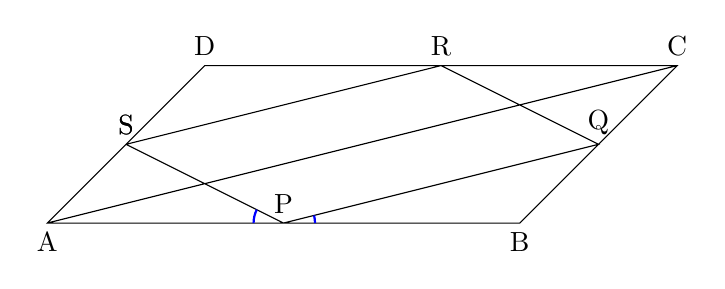
\begin{tikzpicture}[xslant=1,xscale=3,scale=2]
    \draw (0,0) rectangle
          (1,1) coordinate(C) node[above]{C} -- (0,0) coordinate(A) node[below]{A}
          (1,0) coordinate(B) node[below]{B}  
          (0,1) coordinate(D) node[above]{D}
          (0,0.5) coordinate(S) node[above]{S} --(0.5,0) coordinate(P) node[above]{P} --(1,0.5) coordinate(Q) node[above]{Q} --(0.5,1) coordinate(R) node[above]{R} --(0,0.5) coordinate(S) node[above]{S} 
          pic[draw,blue,thick,angle radius=4mm] {angle = B--P--Q}
          pic[draw,blue,thick,angle radius=3.8mm] {angle=S--P--A};
          pic[draw,black,thick,angle radius=3.8mm] {angle=B--Q--P};
  \end{tikzpicture}
\end{document}
}
\caption{Rhombus}
\label{fig:foo}
\end{figure}
From $\triangle{ABC}$ and $\triangle{ADC}$
\begin{align}
PQ || AC \hspace{2pt}\text{and}\hspace{2pt} PQ=\frac{1}{2}AC\\
RS || AC \hspace{2pt}\text{and}\hspace{2pt} RS=\frac{1}{2}AC
\end{align}
from 4 and 5 PQ=RS , PQ||RS 
\begin{align}
 \textit{As}\hspace{6pt} PB=PQ, \angle{2} =\angle{1}
\end{align}
\end{frame}
\begin{frame}
From $\triangle{APS}$ and $\triangle{CQR}$ \\
\begin{itemize}
\item AP=CQ,AS=CR, PS=QR\\
\item From SSS rule
$\triangle{APS} \cong \triangle{CQR}$
\begin{align}
\angle{3} = \angle{4}
\end{align}
\end{itemize}
For AB, BC
\begin{align}
\angle{3}+\angle{SPQ}+\angle{1} = 180\degree
\end{align}
\begin{align*}
\angle{2}+\angle{PQR}+\angle{4}=180\degree
\end{align*}
from 6 and 7 
\begin{align}
\angle{1}+\angle{PQR}+\angle{3}=180\degree
\end{align}
\begin{center}
PS|| PR $\angle{SPQ}+\angle{PQR} =180\degree \implies \angle{SPQ}=90\degree$
\end{center}
\end{frame}
\begin{frame}{Quadrilateral Construction}
\begin{enumerate}
\conti
\item construct a quadrilateral MIST where MI=3.5, IS = 6.5, $\angle{M} = 75\degree , \angle{I} = 105\degree $and $\angle{S} =120\degree$
\seti
\end{enumerate}
\textbf{solution:}
\end{frame}
\begin{frame}{Circle exercises}
\begin{enumerate}
\conti
\item Two circles intersect at two points B and C.
Through B, two line segments ABD and PBQ
are drawn to intersect the circles at A, D and
P, Q respectively. Prove that $\angle{ACP}=\angle{QCD}$
\seti
\end{enumerate}
\textbf{Solution:}
\begin{figure}[!ht]
\resizebox{0.2\linewidth}{!}
{
\documentclass{article}
\usepackage{tikz}
\usetikzlibrary{shapes.geometric,calc,angles,positioning,intersections,quotes,decorations,babel,patterns,fit}
\usepackage{tkz-euclide}
\begin{document}
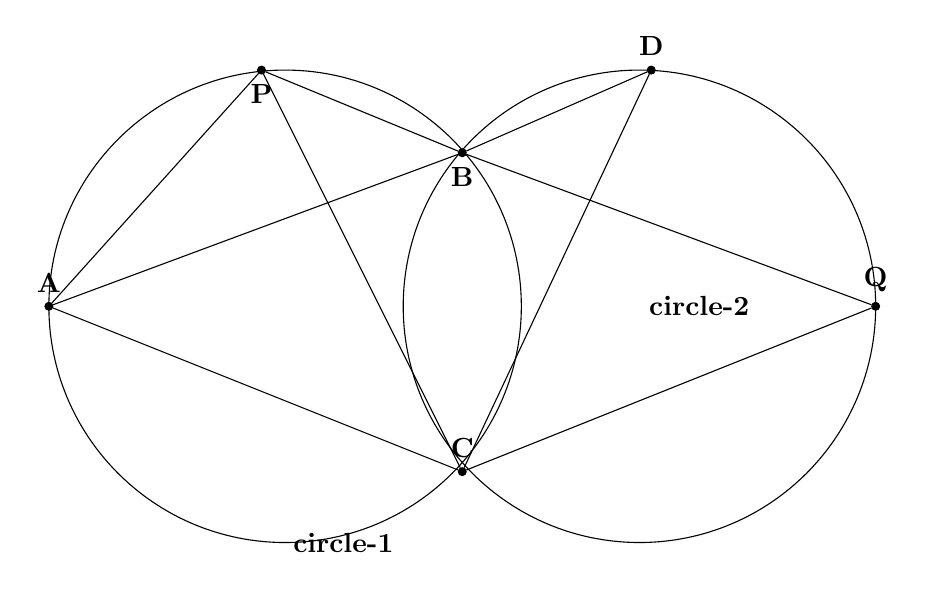
\begin{tikzpicture}[scale =1.5,>=stealth,point/.style = {draw, circle, fill = black, inner sep = 1pt},]
\draw node[left] {$\textbf{circle-1}$}(2,2)circle (2cm)node[right] {$\textbf{circle-2}$} (-1,2) circle (2cm);
\node (A) at (-3,2)[point,label=above :$\textbf{A}$] {};
\node (P) at (-1.2,4)[point,label=below :$\textbf{P}$] {};
\node (B) at (0.5,3.3)[point,label=below :$\textbf{B}$] {};
\node (Q) at (4,2)[point,label=above :$\textbf{Q}$] {};
\node (D) at (2.1,4)[point,label=above :$\textbf{D}$] {};
\node (C) at (0.5,0.6)[point,label=above :$\textbf{C}$] {};
\draw (A)--(P)--(B)--(Q)--(C)--(P);
\draw (A)--(B)--(D)--(C)--(A);
\end{tikzpicture}
\end{document}
}
\caption{Circle}
\label{fig:foo}\textbf{Solution:} 
\end{figure}
From the above figure
\begin{align}
\angle{PBA}=\angle{ACP}\\
\angle{DBQ}=\angle{QCD}\\
\angle{PBA}=\angle{DBQ}
\end{align}\textbf{Solution:} 
from 10,11,12 $\angle{ACP}=\angle{QCD}$
\end{frame}
\begin{frame}{circle constructions}
\begin{enumerate}
\conti 
\item Draw a circle with centre B and radius 6. If C be a point 10 units away from its centre,construct the pair of tangents AC and CD to
the circle.
\seti
\end{enumerate}
\textbf{Solution:} Taking M as centre and MB as radius, draw a circle. 
\begin{figure}[!ht]
\resizebox{0.35\linewidth}{!}
{
\documentclass{article}
\usepackage{tikz}
\usetikzlibrary{shapes.geometric,calc,angles,positioning,intersections,quotes,decorations,babel,patterns,fit}
\usepackage{tkz-euclide}
\begin{document}
\begin{tikzpicture}[scale =0.9,>=stealth,point/.style = {draw, circle, fill = black, inner sep = 1pt},]
\draw (-1,0)circle (6cm);
\node (C) at (10,0)[point,label=above :$C$] {};
\node (A) at (3.5,4)[point,label=below :$A$] {};
\node (B) at (-1,0)[point,label=below :$B$] {};
\node (D) at (3.5,-4)[point,label=below :$D$] {};
\node (M) at (3.5,0)[point,label=above :$\textbf{M}$] {};
\draw (A)--(B)--node[below] {$\textbf{5cm}$}(M)--node[below] {$\textbf{5cm}$}(C)--node[below] {$\textbf{8cm}$}(D)--(B);
\draw (A)--node[below] {$\textbf{8cm}$}(C);
\draw (D)--(M)--(A)--(3.5,9);
\draw (D)--(3.5,-9)	;
\end{tikzpicture}
\end{document}
}
\caption{Circle}
\label{fig:foo}
\end{figure}
python code : https://github.com/d-DP/Codes
\end{frame}

\begin{frame}{Miscellaneous}
\begin{enumerate}
\conti
\item The lengths of two parallel chords of a circle are 6 cm and 8 cm. If the smaller chord is
at distance 4 cm from the centre, what is the
distance of the other chord from the centre?
\end{enumerate}
\textbf{Solution:} 
\begin{figure}[!ht]
\resizebox{0.45\linewidth}{!}
{
\documentclass{article}
\usepackage{tikz}
\usetikzlibrary{shapes.geometric,calc,angles,positioning,intersections,quotes,decorations,babel,patterns,fit}
\usepackage{tkz-euclide}
\begin{document}
\begin{tikzpicture}[scale =0.9,>=stealth,point/.style = {draw, circle, fill = black, inner sep = 1pt},]
\draw (0,0)circle (8cm);
\node (O) at (0,0)[point,label=right :$O$] {};
\node (A) at (-6.2,5)[point,label=below :$A$] {};
\node (B) at (6.2,5)[point,label=below :$B$] {};
\node (C) at (-7,-4)[point,label=below :$C$] {};
\node (D) at (7,-4)[point,label=above :$D$] {};
\node (M) at (0,5)[point,label=above :$M$] {};
\node (N) at (0,-4)[point,label=below :$N$] {};
\draw (A)--node[below] {$\textbf{6cm}$}(B);
\draw (C)--node[left] {$\textbf{8cm}$}(D);
\draw (O)--node[left] {$\textbf{a=4cm}$}(M);
\draw (O)--node[left] {$\textbf{x}$}(N);
\draw (O)--node[below] {$\textbf{b}$}(B);
\draw (O)--node[below] {$\textbf{b}$}(D);
\draw (M)--node[below] {$\textbf{3cm}$}(B);
\draw (N)--node[below] {$\textbf{4cm}$}(D);
\end{tikzpicture}
\end{document}
}
\caption{Circle}
\label{fig:foo}
\end{figure}
\end{frame}
\begin{frame}
Apply Baudhayana theorem for $\triangle{MOB}$ and $\triangle{NOD}$
\begin{align*}
a^2+b^2=(3)^2 \\
x^2+b^2=(4)^2
\end{align*}

\end{frame}
\end{document}